\documentclass{article}[11pt]

\usepackage{amsmath}
\usepackage{graphicx,color,geometry}
\usepackage{hyperref}
\usepackage{amsfonts}
\usepackage{subcaption}

\begin{document}
\title{Numerical solution of Perspective Shape from Shading}
\author{Balaje K \\ Sanath Keshav}
\date{\today}

\maketitle

\section{Mathematical Model}
The shape from shading problems are typically described by Hamilton
Jacobi Equations. Prados et.al established a mathematical model and a
numerical scheme to solve the Shape from Shading problem that
converges to the unique viscosity solution. Refer\cite{prados}. \\

\noindent
The Hamilton Jacobi Equation that governs the Shape from Shading
problem, proposed by Prados\cite{prados} is given by,
\begin{equation}
  -e^{-2v} + J(\mathbf{x})\sqrt{f^2\lvert \nabla v \rvert^2 +
    (\mathbf{x}.\nabla v)^2 + Q(\mathbf{x})^2} = 0 \label{eq:1}
\end{equation}
where $f$ is the focal length, $v = \ln u$
\begin{eqnarray}
J(\mathbf{x}) =
  \frac{I(\mathbf{x})f^2}{Q(\mathbf{x})}\\
  Q(\mathbf{x}) =
  \sqrt{\frac{f^2}{\mathbf{x}^2+f^2}}
\end{eqnarray}

\noindent
$I(\mathbf{x})$ is the intensity image to be given as input,
$\mathbf{x} \in \mathbb{R}^2$, and $u:\mathbb{R}^2\to\mathbb{R}$ is the
depth of the reconstructed image.

\section{Numerical Scheme}
We used a Godunov Type upwinded Numerical scheme to solve the PDE with
Dirichlet Boundary conditions. The description of the scheme is given
below.\\

\noindent
We first add a transient term $u_t$ to the PDE given in \ref{eq:1} 
\begin{equation}
v_t + \left(-e^{-2v} + J(\mathbf{x})\sqrt{f^2\lvert \nabla v \rvert^2 +
	(\mathbf{x}.\nabla v)^2 + Q(\mathbf{x})^2} \right) = 0 \label{eq:2}
\end{equation}
and
solve for $v(x,t)$ till we reach a steady state $\lVert U^{n+1} - U^{n} \rVert < \epsilon$.  We replace the
derivatives in $\lvert \nabla v \rvert^2$ term by the respective upwinded finite
difference formulae as shown below.
\begin{eqnarray}
  \frac{\partial u}{\partial x} \approx D^{x}_{upwind} = \max\left\{\left\lvert
  \max\left\{\ \frac{u_{i,j}-u_{i-1,j}}{h},0\right\} \right\rvert, \left\lvert\min\left\{\ \frac{u_{i+1,j}-u_{i,j}}{h},0\right\} \right\rvert \right\}\\
  \frac{\partial u}{\partial y} \approx D^{y}_{upwind} = \max\left\{\left\lvert
  \max\left\{\ \frac{u_{i,j}-u_{i,j-1}}{h},0\right\} \right\rvert, \left\lvert\min\left\{\ \frac{u_{i,j+1}-u_{i,j}}{h},0\right\} \right\rvert \right\}
\end{eqnarray}

\noindent
For the derivatives in $(\mathbf{x}.\nabla v)^2$ term, we use the same finite difference that was chosen in the previous step. Let us call that $D^x$ and $D^y$. The final explicit numerical scheme that we use is given by,
\begin{equation}
	v_{i,j}^{n+1} = v_{i,j}^n - \Delta t \left(-e^{-2v_{i,j}} + J(x_i,y_j) \sqrt{f^2\left( (D^x_{upwind})^2 + (D^y_{upwind})^2 \right) + \left(x_iD^x + y_jD^y\right)^2 + Q(x_i,y_j)^2} \right)
\end{equation}

\noindent

\section{Results}
We ran our algorithm for a few standard test cases and the results are presented below.
\begin{figure}[h!]
	\begin{subfigure}{0.5\textwidth}
		\centering
		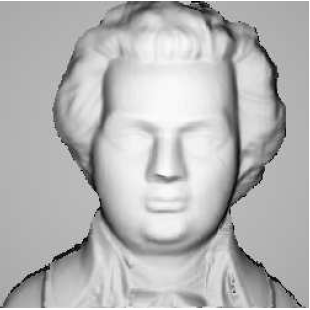
\includegraphics[scale = 0.6]{moz.png}
		\subcaption{The input file for Mozart}
	\end{subfigure}
	\begin{subfigure}{0.5\textwidth}
		\centering
		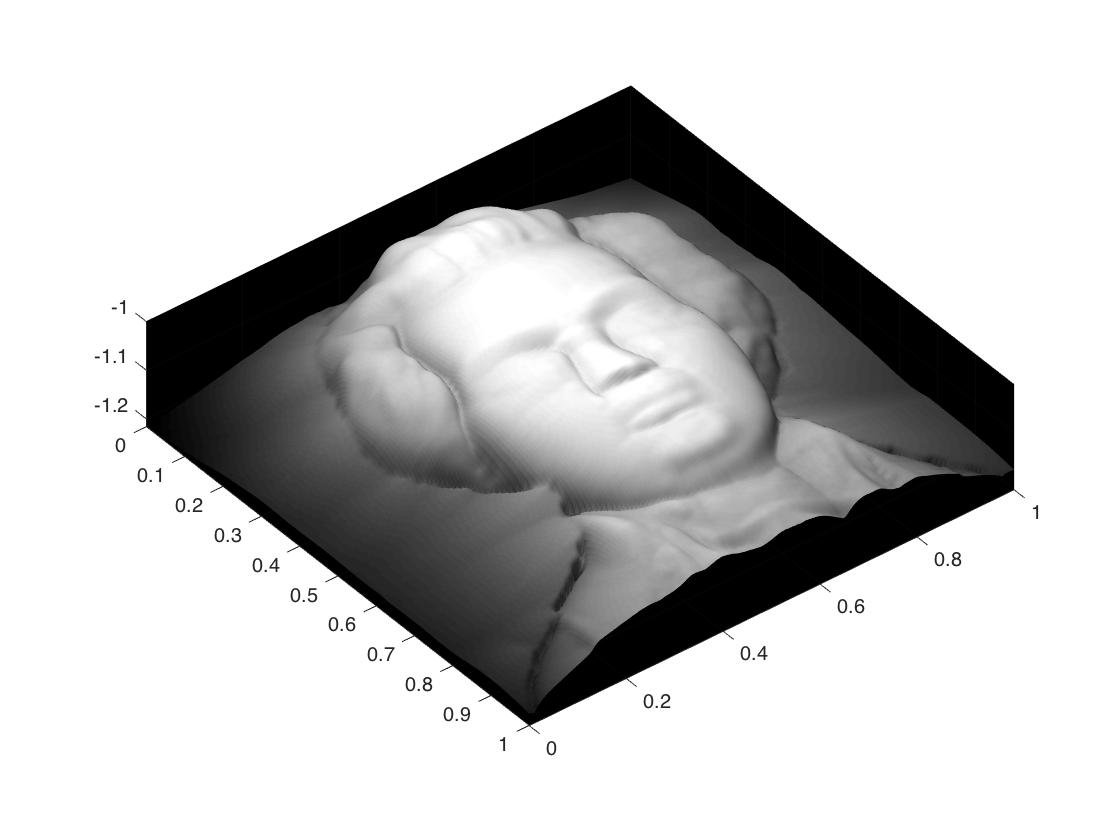
\includegraphics[scale = 0.2]{moz.jpg}
		\subcaption{Reconstructed Image}
	\end{subfigure}
	\caption{Mozart Test. Courtesy \cite{prados}}
	\label{fig:1}
\end{figure}

\begin{figure}[h!]
	\begin{subfigure}{0.5\textwidth}
		\centering
		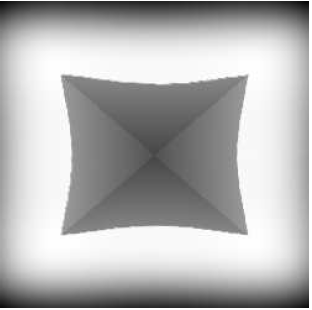
\includegraphics[scale = 0.52]{thing1.png}
		\subcaption{The input file for Trough}
	\end{subfigure}
	\begin{subfigure}{0.5\textwidth}
		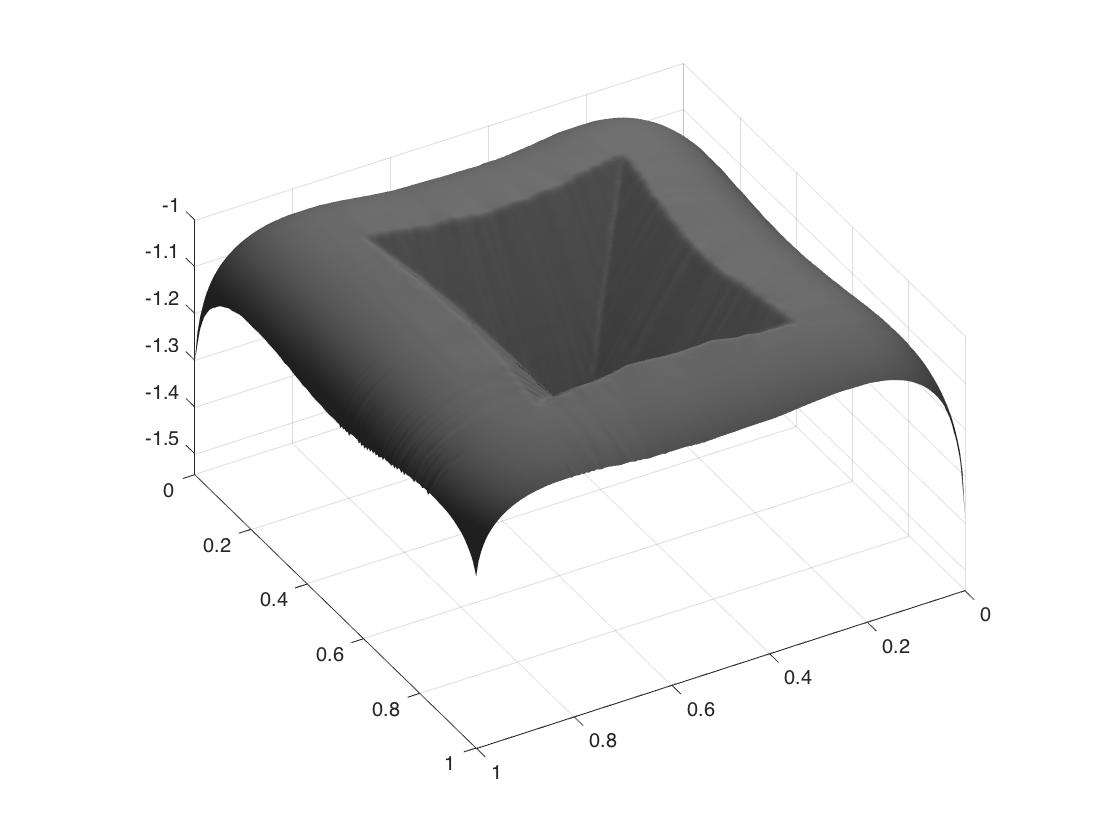
\includegraphics[scale = 0.17]{thing1.jpg}
		\subcaption{Reconstructed Image}
	\end{subfigure}
	\caption{Trough Test. Courtesy \cite{prados}}
	\label{fig:2}
\end{figure}

\noindent
However, for some particular examples, we could not accurately capture the Troughs. We instead get Peaks in place of Troughs, despite including the brighting attenuation term $\frac{1}{r^2}$. See Figure below.
\begin{center}
	\begin{figure}[h!]
	\begin{subfigure}{0.5\textwidth}
		\centering
		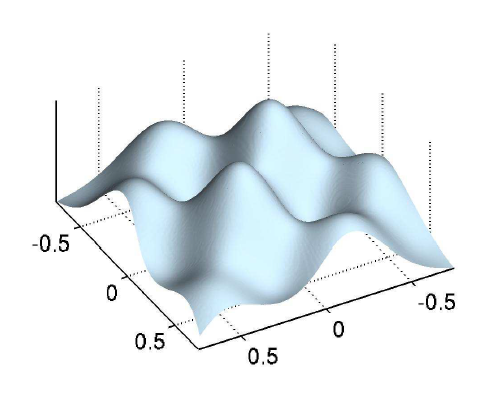
\includegraphics[scale = 1]{gt.png}
		\subcaption{Ground Truth}
	\end{subfigure}
	\begin{subfigure}{0.5\textwidth}
		\centering
		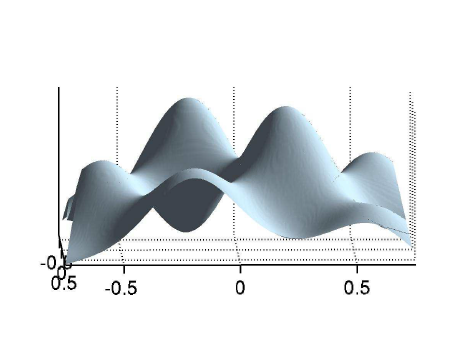
\includegraphics[scale = 1]{gt1.png}
		\subcaption{Ground Truth}
	\end{subfigure}
	\begin{subfigure}{0.5\textwidth}
		\centering
		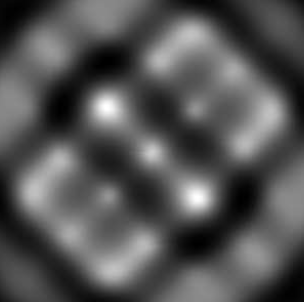
\includegraphics[scale = 1]{thing.png}
		\subcaption{Input Image}
	\end{subfigure}
	\begin{subfigure}{0.5\textwidth}
		\centering
		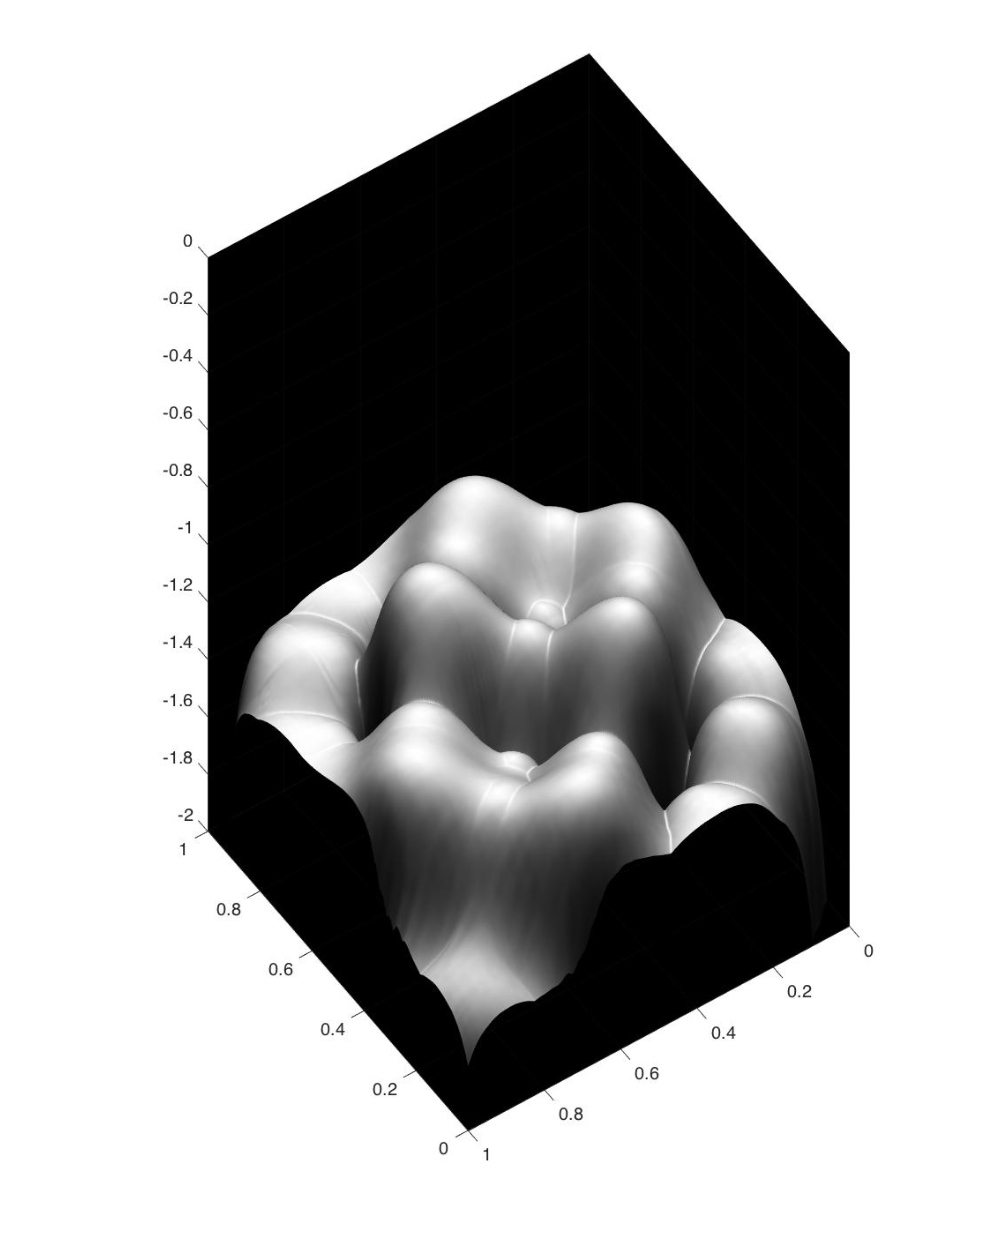
\includegraphics[scale = 0.3]{thing2.png}
		\subcaption{Wrongly Reconstructed Image}
	\end{subfigure}
	\caption{Wrong Reconstruction. ``Ground Truth'' Courtesy \cite{prados}}
\end{figure}
\end{center}

\pagebreak
\noindent
For real life images, the reconstruction yields distorted and elongated 3D shapes, because of incorrectly procured input image intensities. The figure below shows the condition.
\begin{figure}[h!]
	\begin{subfigure}{0.5\textwidth}
		\centering
		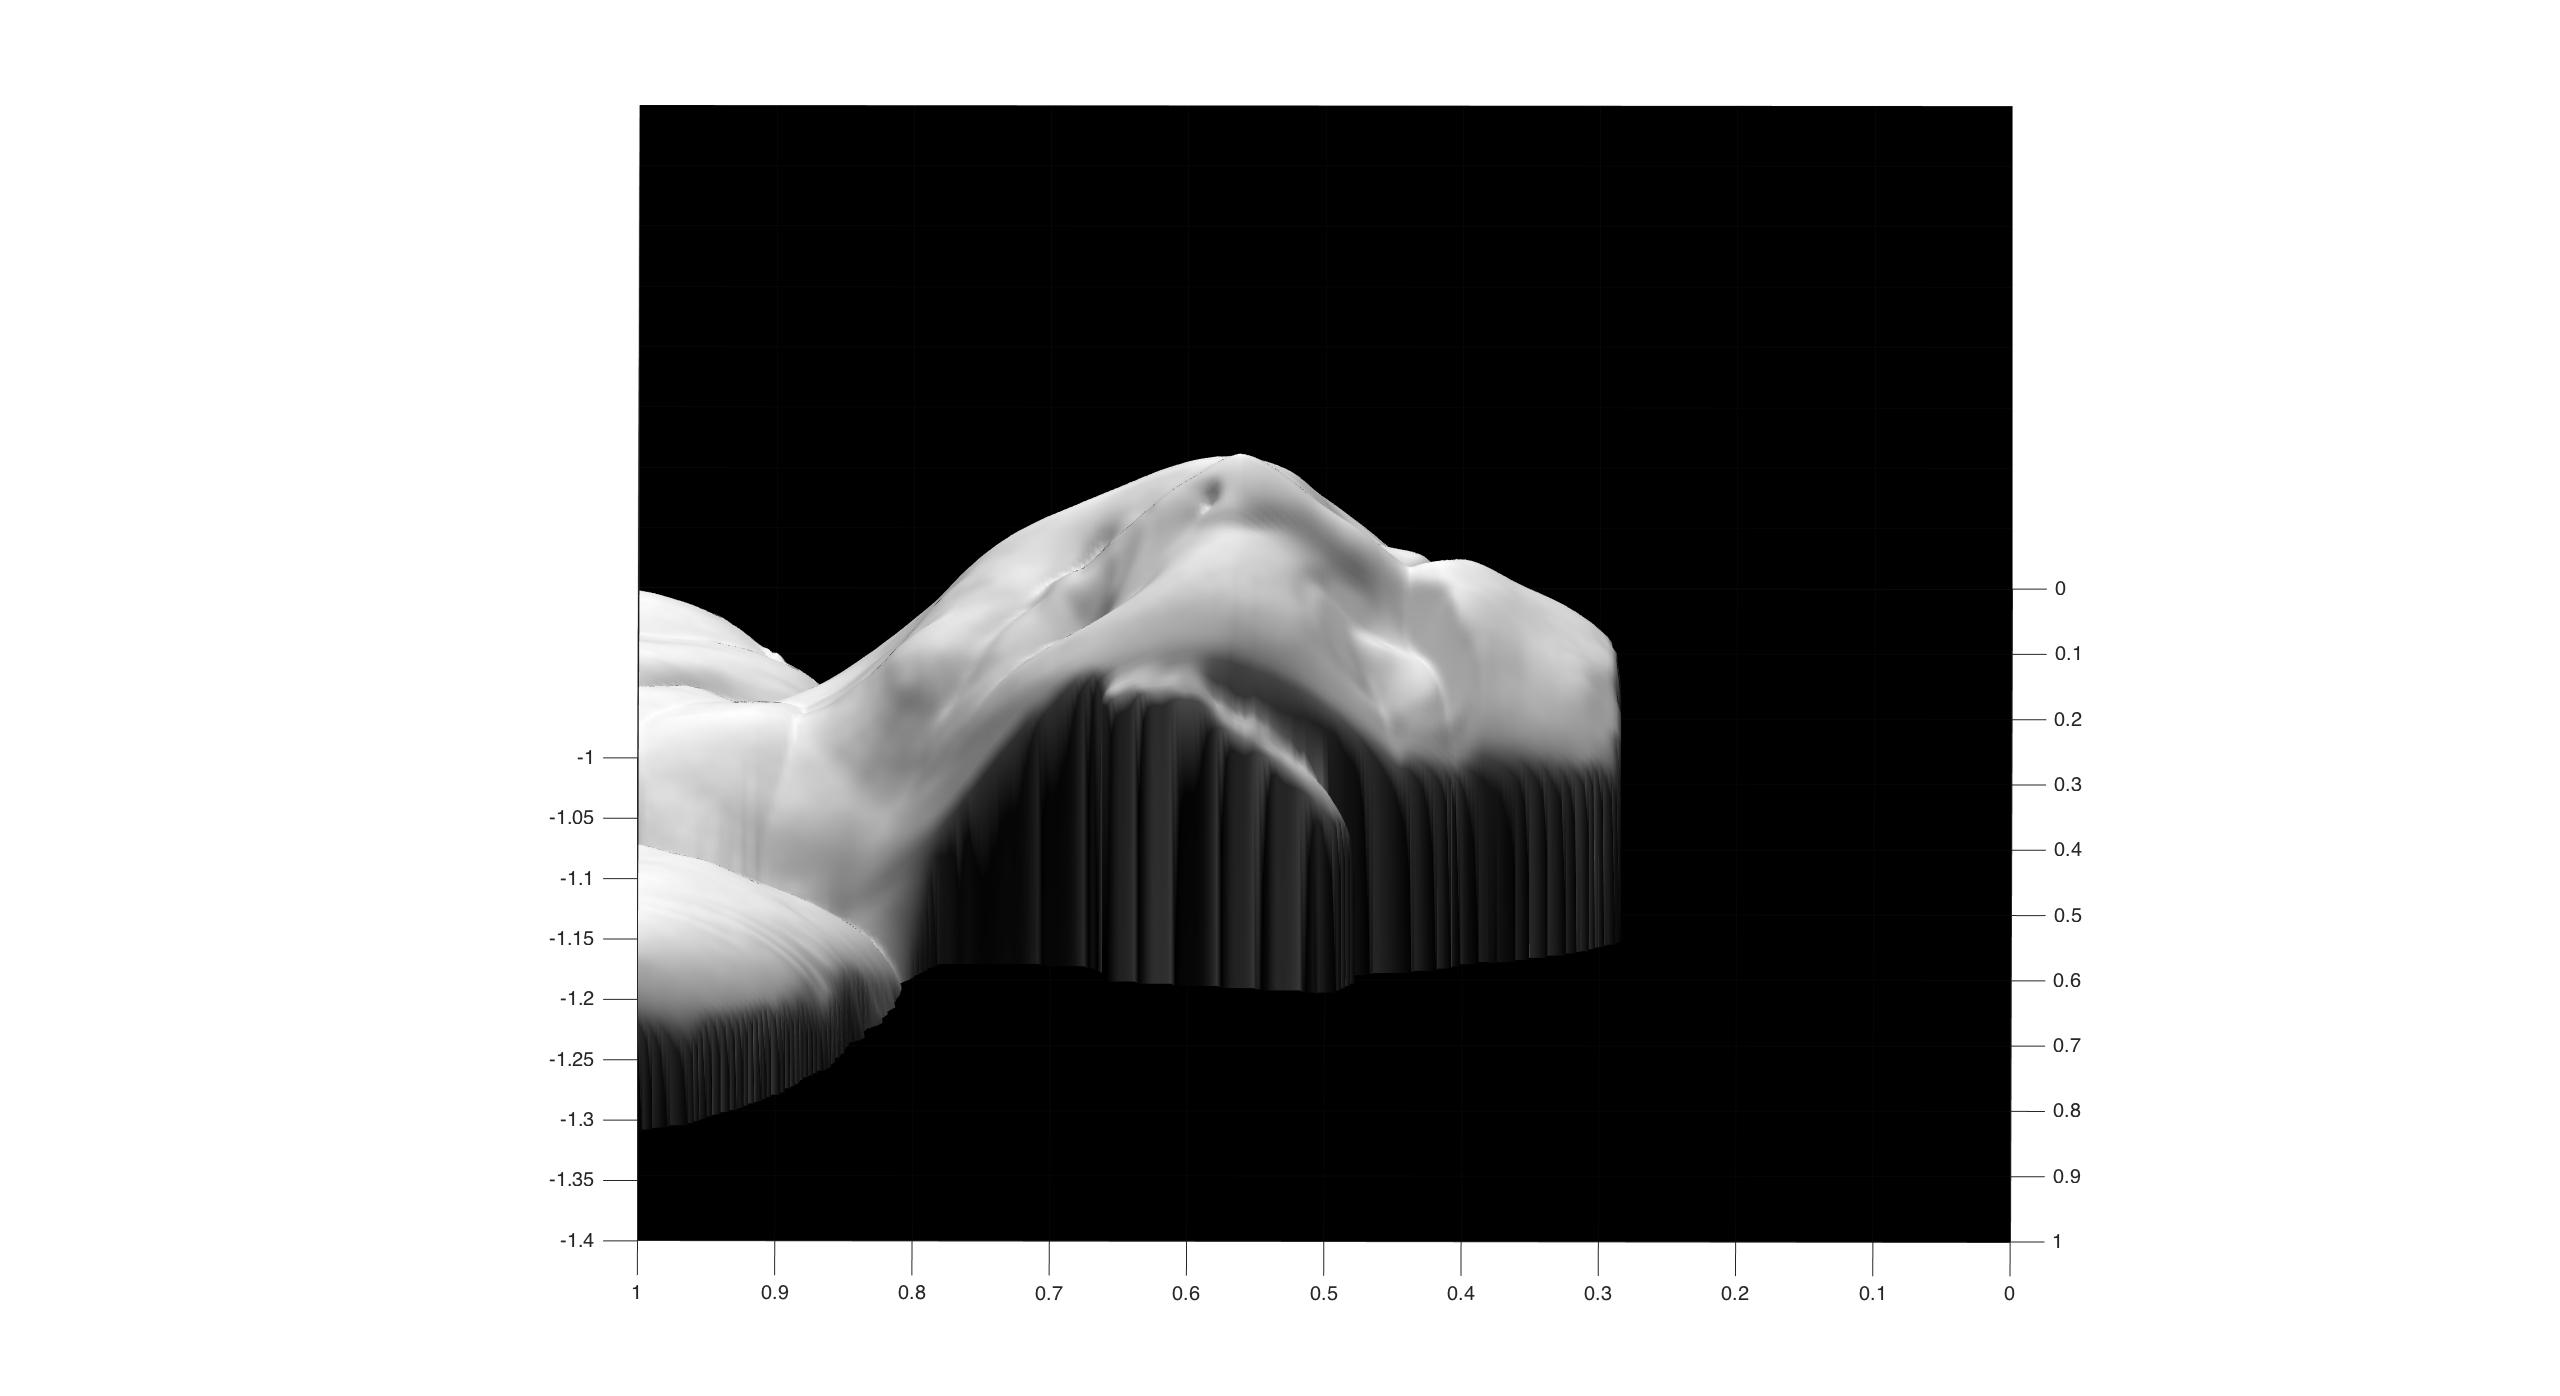
\includegraphics[scale = 0.1]{sanath1.jpg}
		\subcaption{Incorrect Reconstruction}
	\end{subfigure}
	\begin{subfigure}{0.5\textwidth}
		\centering
		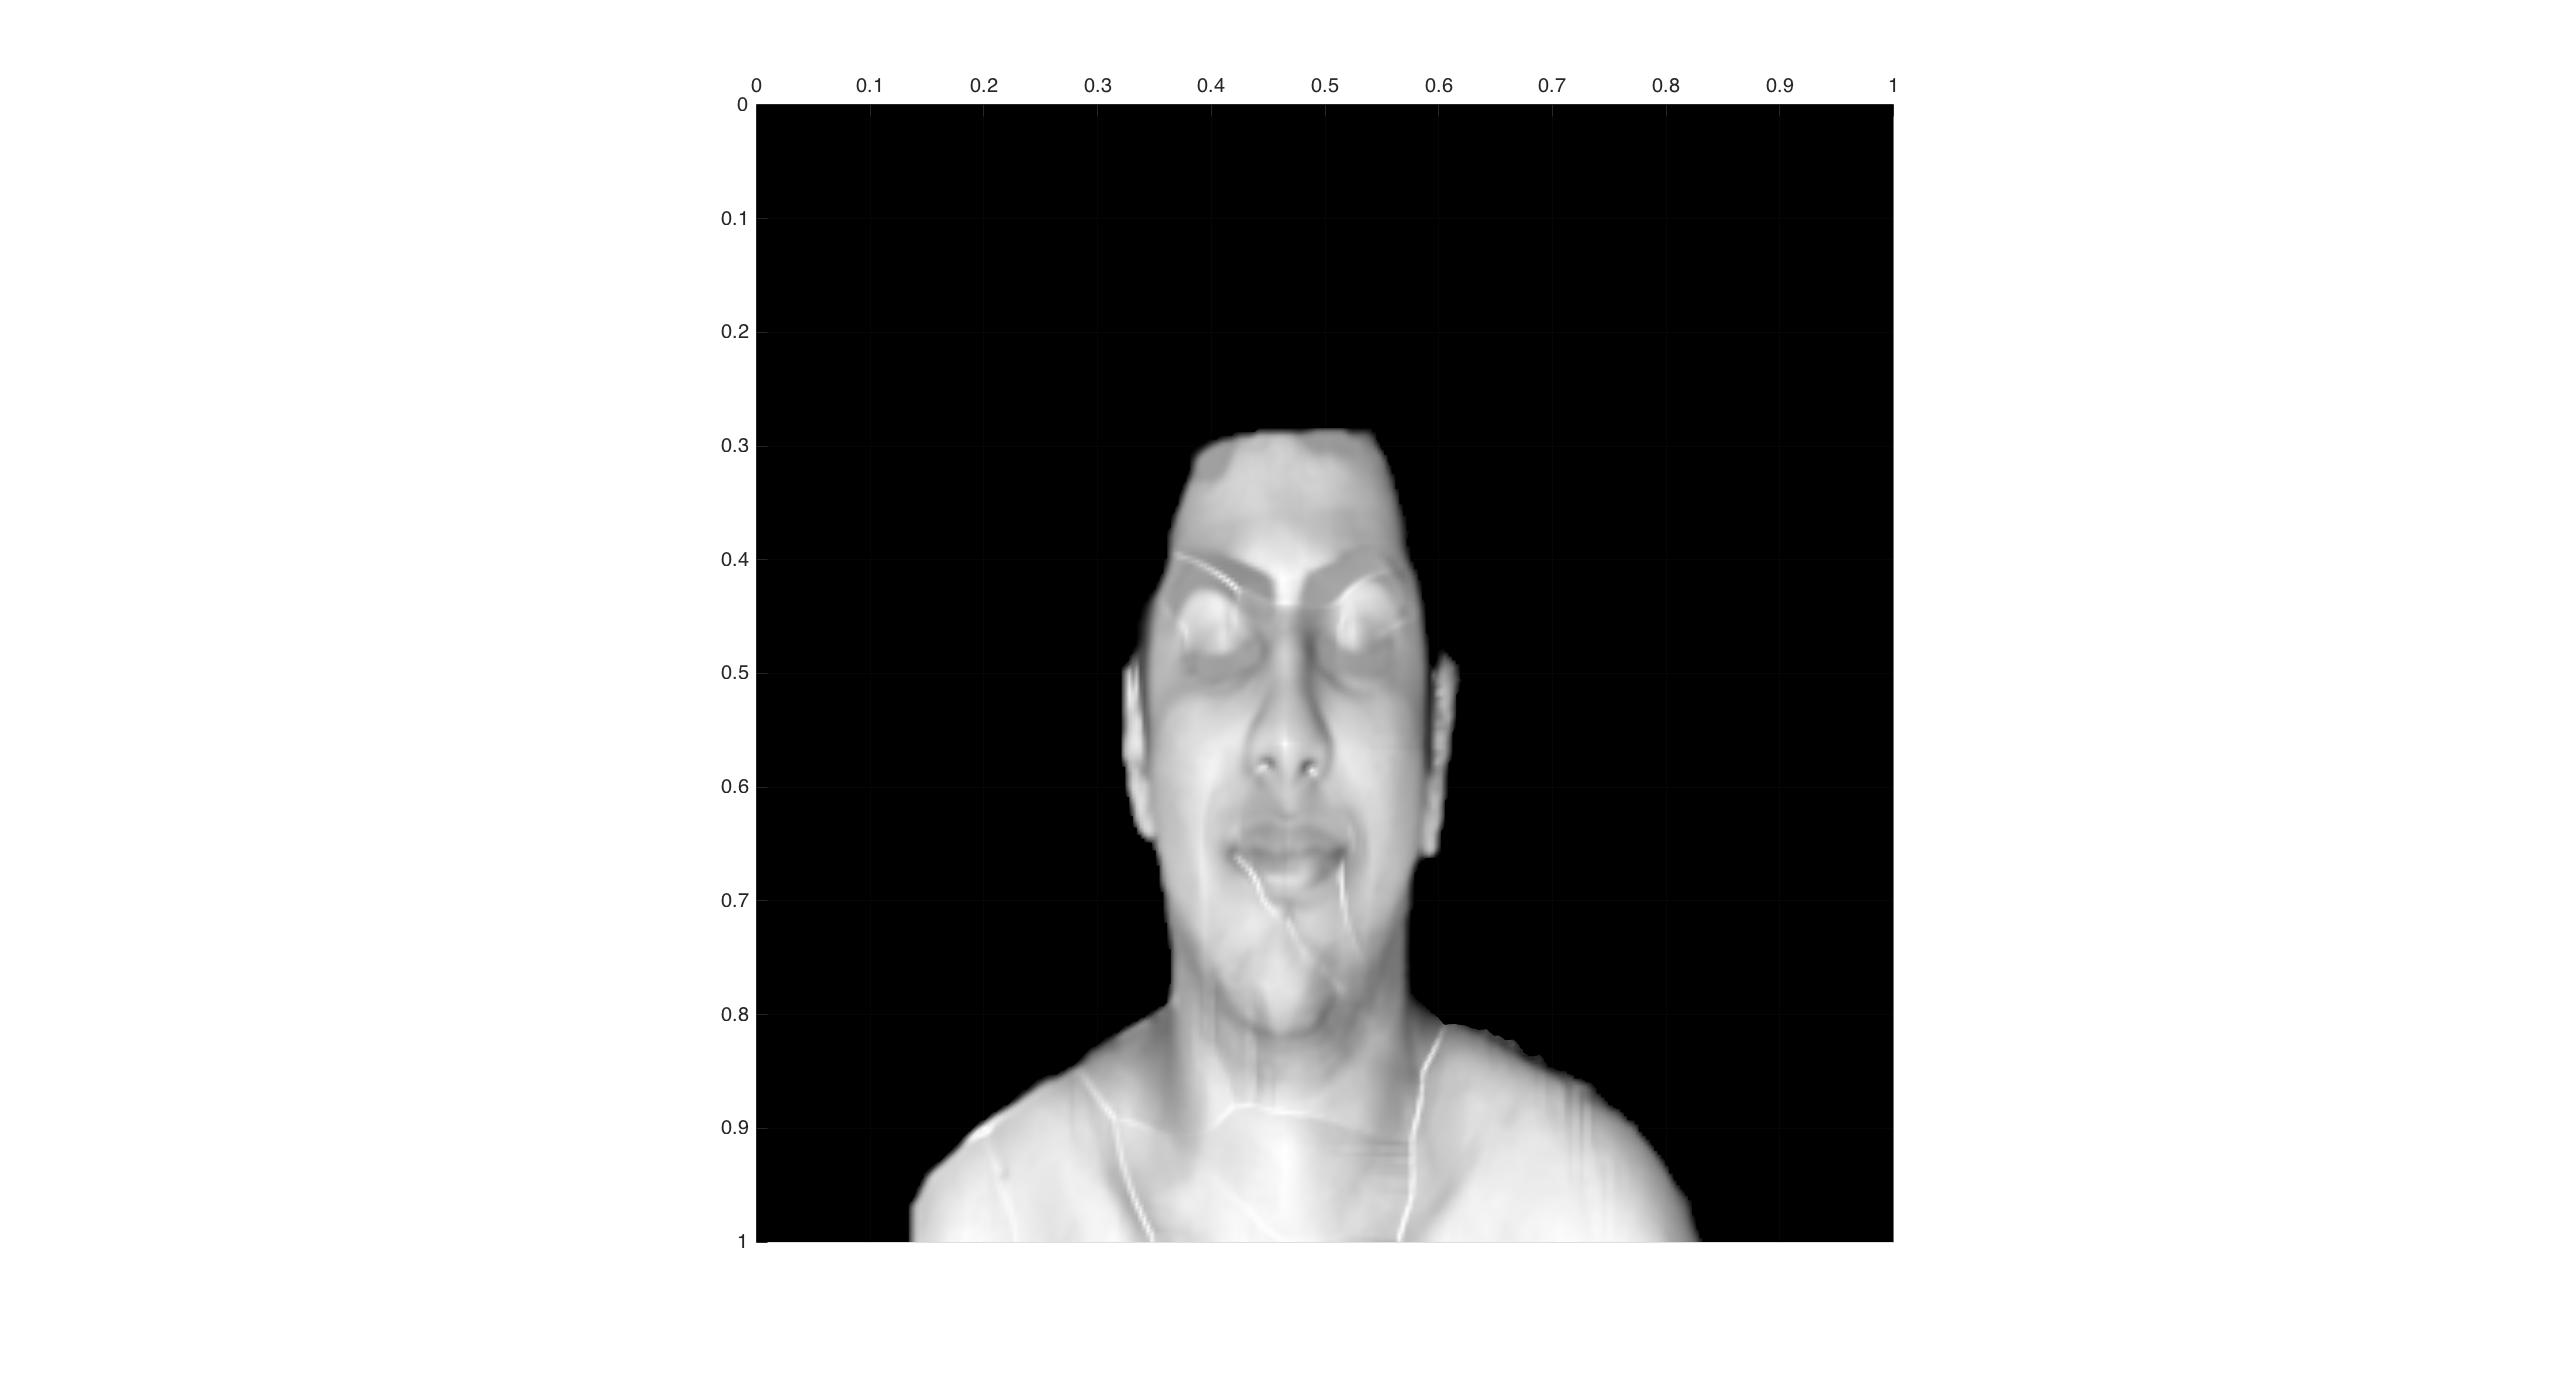
\includegraphics[scale = 0.1]{sanath2.jpg}
		\subcaption{The top view of the reconstruction}
	\end{subfigure}
	\caption{Incorrect Reconstruction}
\end{figure}
\nocite{*}
\bibliographystyle{acm}
\bibliography{biblio}
\end{document}
